\documentclass{article}
\usepackage[UTF8]{ctex} % 添加ctex宏包以支持中文编译
\usepackage{graphicx} % Required for inserting images

\title{DCT-REM}
\author{Yongjian Zhao}
\date{March 2026}
\usepackage{algorithmic}
\usepackage{algorithm}
\usepackage{array}
\usepackage[caption=false,font=normalsize,labelfont=sf,textfont=sf]{subfig}
\usepackage{amsmath,amssymb,amsfonts}

% ---------- 版面与图形 ----------

\usepackage{graphicx}
\usepackage{adjustbox}
\usepackage{textcomp}
\usepackage{siunitx}
\usepackage{textcomp}
\usepackage{stfloats}
\usepackage{url}
\usepackage{verbatim}

\usepackage{array,booktabs,tabularx}
\usepackage{multirow}
\usepackage{hyperref}
\usepackage{adjustbox}
\newcommand{\cmark}{\ding{51}}  % ✓
\newcommand{\xmark}{\ding{55}}  % ✗
\usepackage{pifont}                  % \ding symbols
\newcommand{\fstar}{\ding{72}}       % filled star
\newcommand{\hstar}{\ding{73}}       % hollow star
\newcolumntype{C}[1]{>{\centering\arraybackslash}p{#1}}
\renewcommand{\arraystretch}{1.15}

% ---------- 颜色与引用 ----------
\usepackage{xcolor}                              % ← 必须先加载
\definecolor{labelblue}{RGB}{0,0,180}
\definecolor{numberblue}{RGB}{0,0,180}

\makeatletter                                     % ← 解除 natbib 钩子
\let\NAT@parse\undefined
\makeatother

\usepackage[capitalize]{cleveref}                % ← 后 cleveref
\usepackage[numbers]{natbib}

% ===== cleveref 样式统一 =====
% equation
\crefname   {equation}{\textcolor{labelblue}{公式}}{\textcolor{labelblue}{公式}}
\Crefname   {equation}{\textcolor{labelblue}{公式}}{\textcolor{labelblue}{公式}}
\creflabelformat{equation}{\textcolor{numberblue}{(#2#1#3)}}

% figure
\crefname   {figure}  {\textcolor{labelblue}{图}}     {\textcolor{labelblue}{图}}
\Crefname   {figure}  {\textcolor{labelblue}{图}}     {\textcolor{labelblue}{图}}
\creflabelformat{figure}{\textcolor{numberblue}{#2#1#3}}

% table
\crefname   {table}   {\textcolor{labelblue}{表}}   {\textcolor{labelblue}{表}}
\Crefname   {table}   {\textcolor{labelblue}{表}}   {\textcolor{labelblue}{表}}
\creflabelformat{table}{\textcolor{numberblue}{#2#1#3}}

% algorithm
\crefname   {algorithm}{\textcolor{labelblue}{算法}}{\textcolor{labelblue}{算法}}
\Crefname   {algorithm}{\textcolor{labelblue}{算法}}{\textcolor{labelblue}{算法}}
\creflabelformat{algorithm}{\textcolor{numberblue}{#2#1#3}}

% ---------- 其他 ----------
\hyphenation{op-tical net-works semi-conduc-tor IEEE-Xplore}

\begin{document}

\maketitle
\section{双传感器混合 6-DoF 伺服框架}
\label{sec:6dof_framework}
针对空间环境下的特定血管平面追踪任务 ，本文采用自主设计的机器人光声层析（PAT）系统.该系统将 PAT 探头集成于机械臂末端，用于获取局部血管的高分辨率横截面图像 .由于该任务涉及复杂的六自由度（6-DoF）空间追踪，本文提出了一种基于“宏观引导-微观伺服”的混合控制策略 .

在追踪初始阶段，当目标尚未进入光声成像视野时，系统利用末端搭载的深度相机（Depth Camera）提供宏观全局视野，引导机械臂向目标区域逼近.该过程受两个关键空间条件约束：首先，探头末端需与皮肤表面保持特定的工作距离 $d^*$，该距离由探头的合成焦距严格标定；其次，探头需被引导至目标血管的宏观邻域内 .

\begin{table}[htbp]
    \centering
    \caption{混合系统中的自由度解耦与反馈映射 }
    \label{tab:dof_decoupling}
    \begin{tabularx}{\columnwidth}{XXXX}
        \toprule
        \textbf{DoF 分量} & \textbf{伺服类型} & \textbf{反馈信号来源} & \textbf{控制目标} \\
        \midrule
        $v_x, v_y$ & IBVS & 光声 DCT 特征 $\mathbf{s}(\mathbf{I})$ & 面内横截面平移对齐 \\
        $\omega_z$ & IBVS & 光声 DCT 特征 $\mathbf{s}(\mathbf{I})$ & 面内横截面旋转对齐 \\
        $v_z$ & PBVS & 深度相机 $d$ & 维持恒定工作距离 $d^*$ \\
        $\omega_x, \omega_y$ & PBVS & 深度相机法向量 $\mathbf{n}$ & 面外姿态对齐 \\
        \bottomrule
    \end{tabularx}
\end{table}

当完成初始定位且光声图像成功显现后，系统无缝切换至混合视觉伺服阶段 .为保证所有光声图像均在同一高度平面内采集，深度相机将在全过程中持续主导 $Z$ 轴方向的位置伺服，以维持恒定的工作距离 $d^*$ .具体而言，系统采用了如\cref{tab:dof_decoupling}所示的解耦策略：面内分量（$v_x, v_y, \omega_z$）由基于光声 DCT 特征 $\mathbf{s}(\mathbf{I})$ 的基于图像的视觉伺服（IBVS）控制；面外分量（$\omega_x, \omega_y, v_z$）则由基于深度信息的基于位置的视觉伺服（PBVS）闭环接管.

\subsection{光声平面外的位置伺服理论推导}
\label{sec:out_of_plane}
\setlength{\abovedisplayskip}{6pt}
\setlength{\belowdisplayskip}{6pt}
设 $\{P\}$ 为探头坐标系，$z_P$ 轴取为探头声束法向。深度相机估计得到皮肤表面法向量
\[
\mathbf{n} = [n_x, n_y, n_z]^\top
\]
并将其表达在 $\{P\}$ 中。期望情况下，探头法向与皮肤法向对齐，因此设期望法向为
\begin{equation}
\mathbf{n}^{*} =
\begin{bmatrix}
0 \\ 0 \\ 1
\end{bmatrix}.
\end{equation}

同时，设 $d$ 为沿 $z_P$ 方向测得的探头到皮肤表面的有符号距离，期望工作距离为 $d^*$。定义距离误差
\begin{equation}
e_d = d - d^* .
\end{equation}

对姿态误差，采用由表面法向构造的局部姿态误差。先定义三维叉乘误差
\begin{equation}
\mathbf{e}_n = \mathbf{n} \times \mathbf{n}^{*}
=
\begin{bmatrix}
n_y \\ -n_x \\ 0
\end{bmatrix}.
\end{equation}

由于偏航自由度 $\omega_z$ 由面内伺服单独控制，这里只保留与面外姿态相关的前两项，定义
\begin{equation}
\mathbf{e}_{\omega} =
\begin{bmatrix}
n_y \\ -n_x
\end{bmatrix}.
\end{equation}

于是面外误差向量定义为
\begin{equation}
\mathbf{e}_{out}
=
\begin{bmatrix}
e_d \\ \mathbf{e}_{\omega}
\end{bmatrix}
=
\begin{bmatrix}
d - d^* \\ n_y \\ -n_x
\end{bmatrix}.
\end{equation}

下面补上误差动力学。约定 $v_z$ 的正方向与 $d$ 的增大方向一致，则有
\begin{equation}
\dot{e}_d = \dot{d} = v_z .
\end{equation}

对于法向量，若表面在世界系中静止，则其在探头系中的变化满足
\begin{equation}
\dot{\mathbf{n}} = [\mathbf{n}]_{\times}\,\boldsymbol{\omega},
\end{equation}
其中 $\boldsymbol{\omega} = [\omega_x, \omega_y, \omega_z]^\top$，$[\mathbf{n}]_{\times}$ 为反对称矩阵。在线性化工作点 $\mathbf{n} = \mathbf{n}^{*} = [0,0,1]^\top$ 附近，有
\begin{equation}
\dot{n}_x \approx -\omega_y, \qquad \dot{n}_y \approx \omega_x .
\end{equation}

因此
\begin{equation}
\dot{\mathbf{e}}_{\omega}
=
\begin{bmatrix}
\dot{n}_y \\ -\dot{n}_x
\end{bmatrix}
\approx
\begin{bmatrix}
\omega_x \\ \omega_y
\end{bmatrix}.
\end{equation}

将式(6)与上式合并，可得局部线性化的面外误差模型
\begin{equation}
\dot{\mathbf{e}}_{out} = \mathbf{L}_{out}\,\mathbf{v}_{out}, \qquad
\mathbf{v}_{out} =
\begin{bmatrix}
v_z \\ \omega_x \\ \omega_y
\end{bmatrix}, \qquad
\mathbf{L}_{out} \approx \mathbf{I}_3 .
\end{equation}

于是采用如下局部 PBVS 控制律：
\begin{equation}
\mathbf{v}_{out} = -\boldsymbol{\Lambda}_{out}\,\mathbf{e}_{out}, \qquad
\boldsymbol{\Lambda}_{out} = \mathrm{diag}(\lambda_d, \lambda_{\omega}, \lambda_{\omega}),
\qquad \lambda_d > 0,\ \lambda_{\omega} > 0 .
\end{equation}
\label{sec:algorithm}

本文提出了一种基于离散余弦变换（DCT）的视觉伺服框架，以在特定的光声（PA）成像约束下鲁棒地提取和控制视觉特征.本节首先简要回顾了标准频谱变换的集成，随后详细阐述了我们的核心创新：针对光声成像几何特性优化的频域交互矩阵公式，并最终推导出一个混合 6-DoF 双传感器伺服框架——该框架利用 Intel Depth camera 深度相机实现了鲁棒的光声平面外（out-of-plane）运动补偿.

\subsubsection{频谱特征表示}
\label{sec:Spectral_Feature_Representation}

传统的基于图像的视觉伺服（IBVS）通过最小化当前传感器数据与期望目标配置之间的特征空间差异来调节机器人的运动.然而，传统的IBVS依赖于空间像素强度，当应用于医学超声和光声成像时，其表现出极高的噪声敏感性，且收敛域受到严重限制.由于受限于激光的帧率和非平稳的电磁干扰，光声视觉伺服面临的挑战进一步加剧.

为了克服这些特定模态的限制，我们的方法避开了空间强度特征，直接将光声感兴趣区域（ROI）转换至频域.利用成熟的二维离散余弦变换（DCT）\cite{ahmed2006discrete}，我们将空间强度映射为频率系数矩阵.通过采用标准的Z字形扫描协议（如图\Cref{fig:feature_construction}(c)所示），我们优先保留低频分量，从而提取出紧凑的视觉特征向量 \(\boldsymbol{s}(u,v) \in \mathbb{R}^K\).这种频谱截断本质上充当了一个低通滤波器（如图\Cref{fig:DCT_transform}所示），在保留宏观血管拓扑结构的同时，滤除了原始光声信号中特征性的高频干扰.


Consider a photoacoustic image region of interest (ROI) represented by pixel intensities \(\boldsymbol{I}(x, y)\) with dimensions \(M \times N\). The two-dimensional DCT-II transform maps this spatial-domain representation to the frequency domain through \cite{ahmed2006discrete}:
\begin{equation}
\boldsymbol{F}_{uv} = \sum_{y=0}^{N-1} \sum_{x=0}^{M-1} \phi_{uv}(x,y)\,\boldsymbol{I}(x,y),
\label{2D-DCT-equation}
\end{equation}
\begin{figure}[!htb]
    \centering
    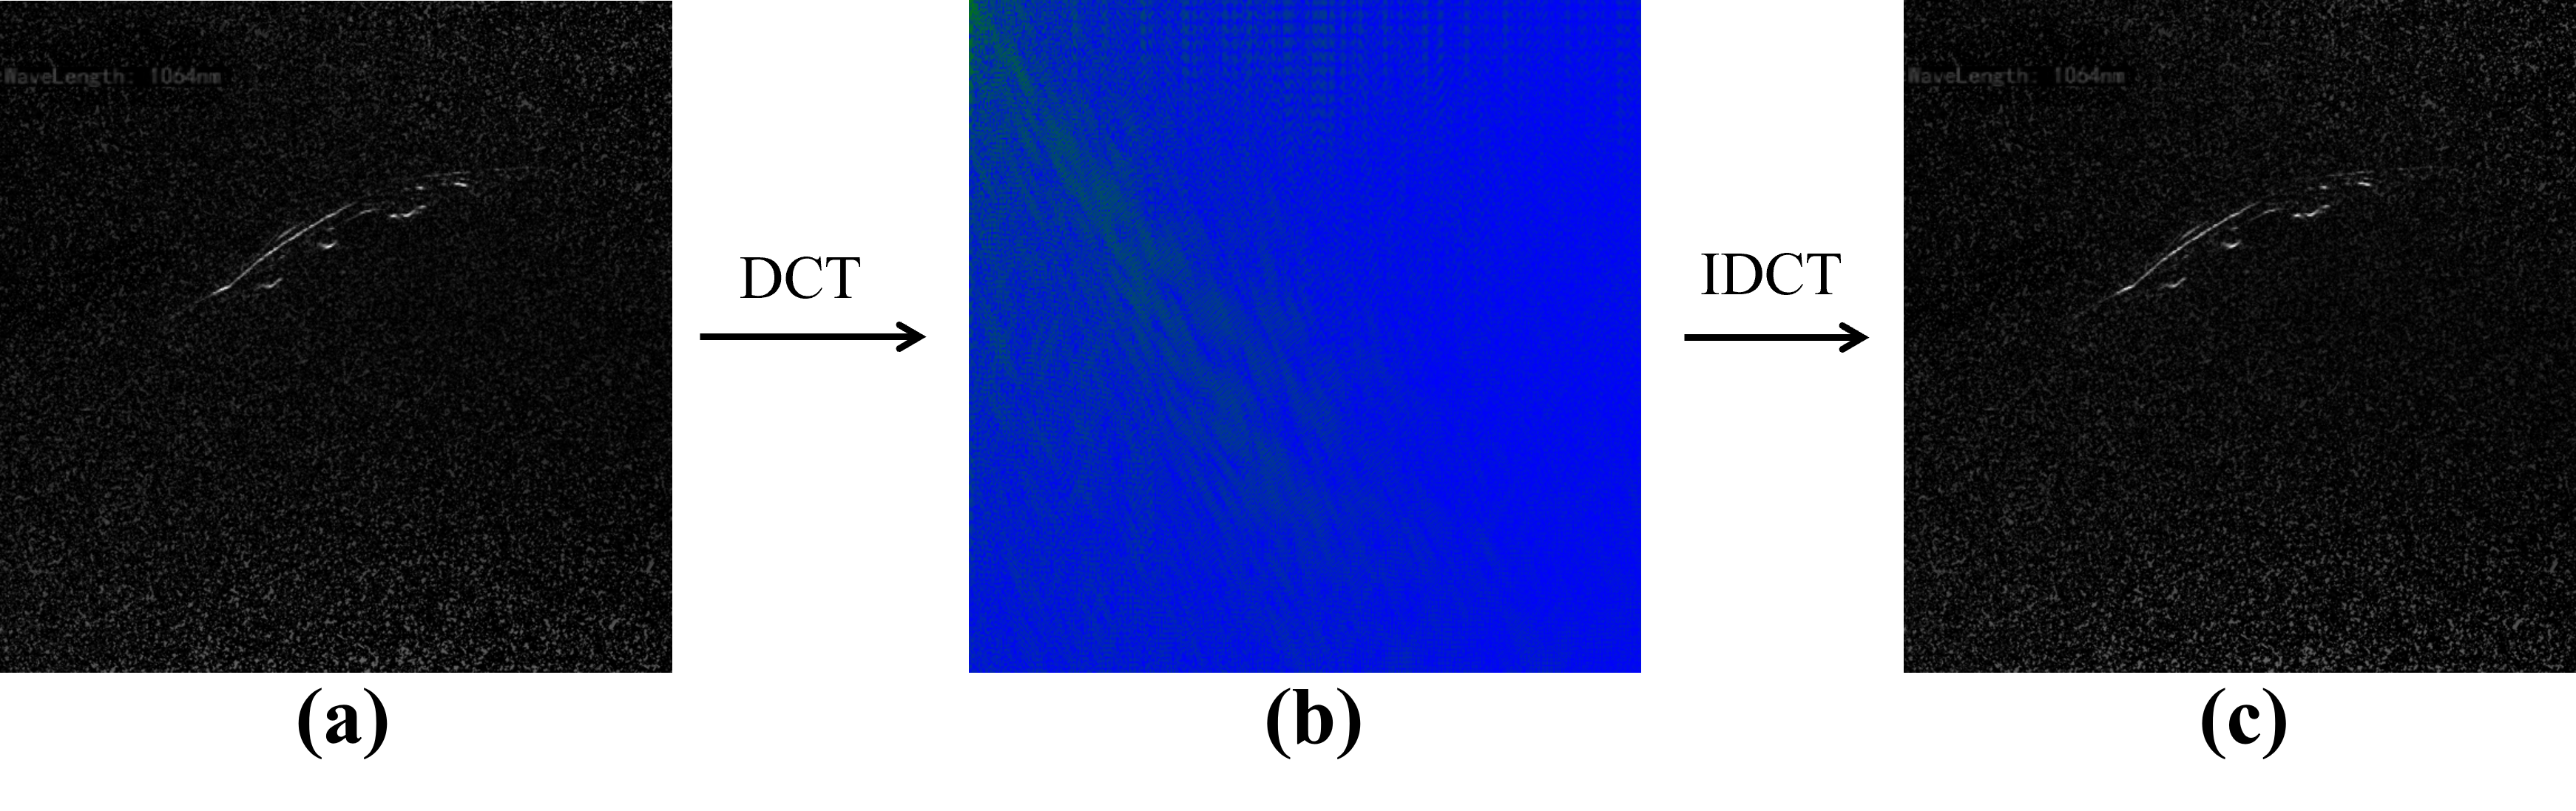
\includegraphics[width=\columnwidth]{graph/IDCT_new.png}
    \caption{Spectral decomposition and reconstruction via Discrete Cosine Transform: 
    (a) Original spatial-domain vascular image \(\boldsymbol{I}(x, y)\), 
    (b) Frequency-domain coefficient matrix \(\boldsymbol{F}(u, v)\) showing characteristic energy compaction in low-frequency quadrant, 
    (c) Perfect reconstruction through IDCT validating transformation integrity and noise preservation properties}
    \label{fig:DCT_transform}
\end{figure}


其中，$\phi_{uv}(x,y)$是基函数，The transformation can be expressed in matrix formulation as:
\begin{equation}
\boldsymbol{F} = \boldsymbol{C}_M \boldsymbol{I} \boldsymbol{C}_N^T,
\end{equation}
where \(\boldsymbol{C}_M\) and \(\boldsymbol{C}_N\) are orthogonal transform matrices of sizes \(M\) and \(N\) respectively. 

This coordinate transformation preserves all image information, enabling perfect reconstruction via the inverse DCT (IDCT) as demonstrated in \Cref{fig:DCT_transform}(c). While IDCT serves primarily for visualization in this context, partial coefficient reconstruction introduces approximation errors \cite{kleinman1962nonlinear} (see \Cref{fig:spectral_reconstruction}(c)). The DCT coefficients \(\boldsymbol{F}(u,v)\) therefore constitute effective visual features, replacing raw pixel intensities in the servo framework.

\begin{figure*}[htbp]
    \centering
    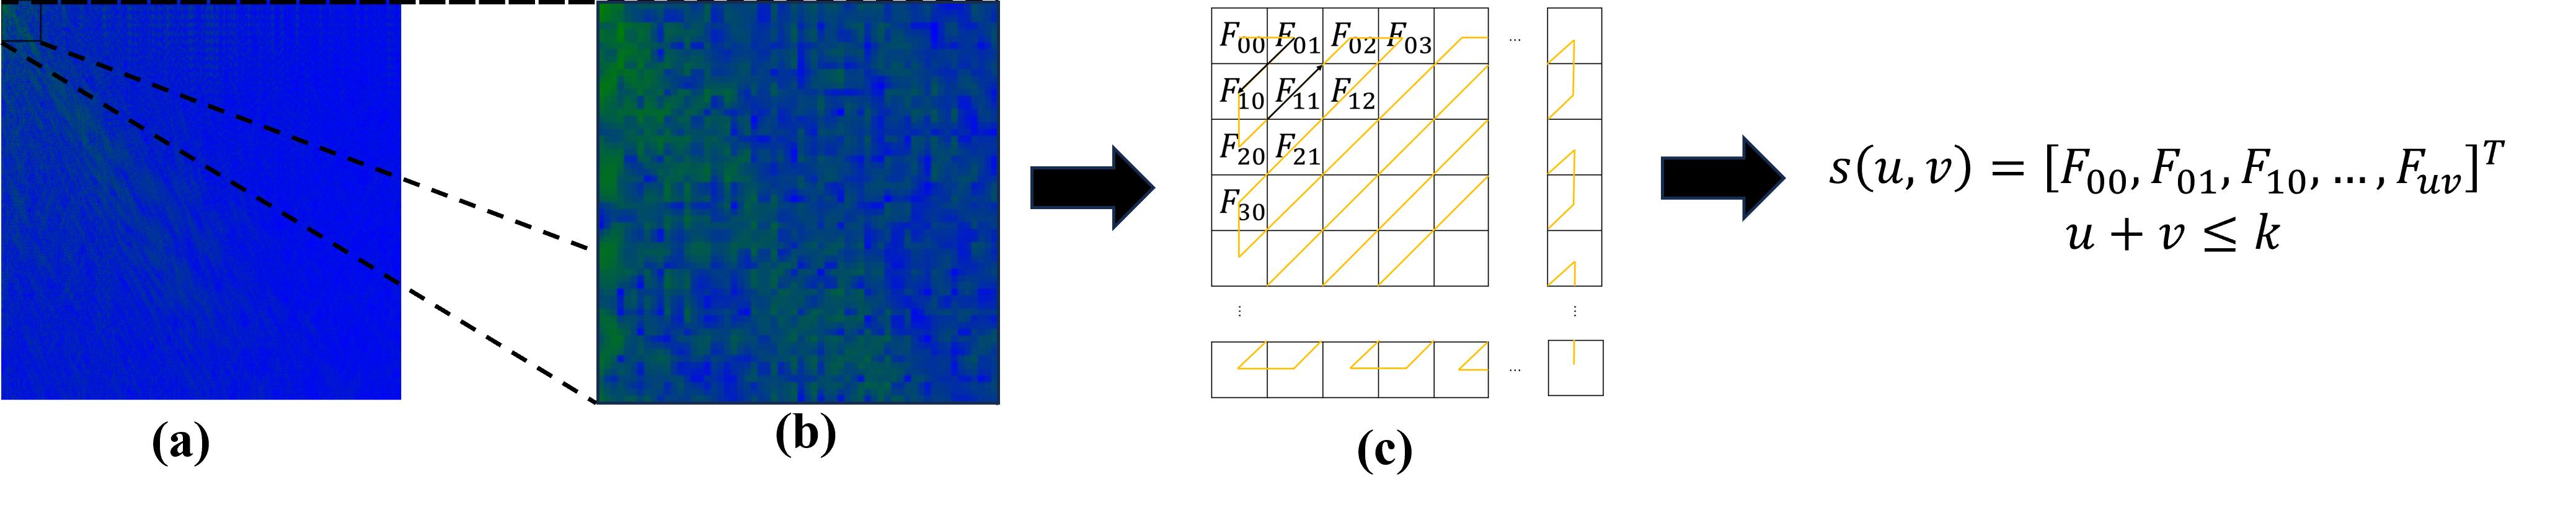
\includegraphics[width=\columnwidth]{graph/spatial calibration.png}
    \caption{Frequency-domain visual feature construction methodology: 
    (a) 2D DCT coefficient spectrum showing spectral energy concentration in low-frequency quadrant (\(u,v < 5\)), 
    (b) Magnified visualization of low-frequency region (\(0 \leq u,v \leq 15\)) demonstrating energy compaction property, 
    (c) Zigzag scanning protocol selecting coefficients satisfying \(u + v \leq k\) to construct compressed feature vector:  
    \(\boldsymbol{s}(u,v) = [F_{00}, F_{01}, F_{10}, \dots, F_{uv}]^\top \in \mathbb{R}^K\)}
    \label{fig:feature_construction}
\end{figure*}

接下来，我们建立了一种利用 DCT 系数的紧凑特征表示方法.对于一个频率索引为 \(u \in [0, M-1]\)、\(v \in [0, N-1]\) 的 \(M \times N\) 数字图像 \(\boldsymbol{I}(x,y)\)，根据 \Cref{2D-DCT-equation} 计算第 \(K\) 阶矩系数（其中 \(K = u + v\)）.视觉特征向量构建如下：
\begin{equation}
\boldsymbol{s}(u, v) = \left[F_{00}, F_{01}, F_{10}, \dots, F_{uv}\right]^T, \quad u + v \le K,
\label{visual feature}
\end{equation}
其中每个 \(F_{uv}\) 均由 DCT 矩阵计算得出.这种基于系数的表示方法在保持视觉识别和跟踪应用判别力的同时，提供了高效的特征编码.

\subsection{DCT 系数排序与动态特征维数选择}
\label{secdynamic coeff}
\begin{equation}
\mathbf{s}_{full} \in \mathbb{R}^{K_{\max}}, \qquad
\mathbf{s}^{*}_{full} \in \mathbb{R}^{K_{\max}} .
\end{equation}

定义固定维度上的全特征误差
\begin{equation}
\mathbf{e}_{full} = \mathbf{s}_{full} - \mathbf{s}^{*}_{full} .
\end{equation}

定义用于调节特征维数的归一化均方误差为
\begin{equation}
\bar{e}_s = \frac{1}{K_{\max}}\|\mathbf{e}_{full}\|_2^2, \qquad
\bar{e}_{s,0} = \frac{1}{K_{\max}}\|\mathbf{e}^{0}_{full}\|_2^2 .
\end{equation}

令自适应调节因子为
\begin{equation}
\eta = \frac{\bar{e}_{s,0}}{\bar{e}_{s,0} + \lambda_{\eta}\bar{e}_s}, \qquad \lambda_{\eta} > 0 .
\end{equation}
则 $\eta \in (0,1]$，并且当误差减小时，$\eta$ 单调增大。

据此定义当前参与控制的特征维数
\begin{equation}
K = \operatorname{clip}\!\left(
\operatorname{round}\!\left((K_{\max} - K_{\min})\eta + K_{\min}\right),
K_{\min},
K_{\max}
\right).
\end{equation}

再定义前 $K$ 维选择矩阵 $\mathbf{P}_K \in \mathbb{R}^{K \times K_{\max}}$，于是实际参与控制的特征与误差为
\begin{equation}
\mathbf{s} = \mathbf{P}_K \mathbf{s}_{full}, \qquad
\mathbf{s}^{*} = \mathbf{P}_K \mathbf{s}^{*}_{full}, \qquad
\mathbf{e}_s = \mathbf{P}_K \mathbf{e}_{full} .
\end{equation}

这样一来，$\bar{e}_s$ 的计算始终基于固定维度 $K_{\max}$，而控制律仅作用于前 $K$ 维特征，定义是闭合的，不再出现循环依赖。自适应增加从低频到中频的 DCT 系数，通常有助于改善局部雅可比的信息丰富度，从而提升 $\mathbf{L}_{PA}$ 满列秩的可能性；但在强对称、低纹理或弱对比场景下，仍可能出现秩退化，因此该条件仍需通过特征选择与初始化共同保证。
\subsubsection{面向光声优化的交互矩阵构建}
\label{sec:PA-Optimized_Interaction_Matrix}
\begin{equation}
\mathbf{v}_{in} =
\begin{bmatrix}
v_x \\ v_y \\ \omega_z
\end{bmatrix}.
\end{equation}

在正交投影近似下，物理平面坐标 $(X,Y)$ 与像素坐标 $(u,v)$ 的关系为
\begin{equation}
u = \alpha_u X + u_0, \qquad
v = \alpha_v Y + v_0 .
\end{equation}

设光声图像 ROI 为 $I(u,v,t)$，其二维 DCT 系数定义为
\begin{equation}
F_{pq}(t) = \sum_{u=0}^{M-1}\sum_{v=0}^{N-1}\phi_{pq}(u,v)\,I(u,v,t),
\end{equation}
其中 $\phi_{pq}(u,v)$ 为二维 DCT 基函数。

对上式关于时间求导，得
\begin{equation}
\dot{F}_{pq} = \sum_{u=0}^{M-1}\sum_{v=0}^{N-1}\phi_{pq}(u,v)\,\dot{I}(u,v,t).
\end{equation}

在局部亮度恒定假设下，有
\begin{equation}
\dot{I}(u,v,t) = -\nabla I(u,v,t)^{\top}\dot{\mathbf{p}}(u,v,t), \qquad
\nabla I =
\begin{bmatrix}
\partial_u I \\ \partial_v I
\end{bmatrix},
\end{equation}
其中 $\dot{\mathbf{p}} = [\dot{u}, \dot{v}]^\top$ 为像素速度。

对面内自由度 $(v_x,v_y,\omega_z)$，正交投影下的像素雅可比写为
\begin{equation}
\dot{\mathbf{p}} = \mathbf{J}_{p}(u,v)\,\mathbf{v}_{in}, \qquad
\mathbf{J}_{p}(u,v) =
\begin{bmatrix}
\alpha_u & 0 & -(v-v_0) \\
0 & \alpha_v & (u-u_0)
\end{bmatrix}.
\end{equation}

将其代入局部亮度恒定关系，得
\begin{equation}
\dot{I}(u,v,t) = -\nabla I(u,v,t)^{\top}\mathbf{J}_{p}(u,v)\,\mathbf{v}_{in}.
\end{equation}

再代入 DCT 系数时间导数，可得单个 DCT 系数的交互行向量
\begin{equation}
\dot{F}_{pq} = \mathbf{L}_{F_{pq}}\,\mathbf{v}_{in},
\end{equation}
其中
\begin{equation}
\mathbf{L}_{F_{pq}}
=
-\sum_{u=0}^{M-1}\sum_{v=0}^{N-1}
\phi_{pq}(u,v)\,\nabla I(u,v,t)^{\top}\mathbf{J}_{p}(u,v)
\in \mathbb{R}^{1\times 3}.
\end{equation}

将上式展开，可得
\begin{equation}
\mathbf{L}_{F_{pq}} =
\begin{bmatrix}
L_x(pq) & L_y(pq) & L_{\omega_z}(pq)
\end{bmatrix},
\end{equation}
其中
\begin{equation}
L_x(pq) = -\alpha_u \sum_{u,v}\phi_{pq}(u,v)\,\partial_u I(u,v,t),
\end{equation}
\begin{equation}
L_y(pq) = -\alpha_v \sum_{u,v}\phi_{pq}(u,v)\,\partial_v I(u,v,t),
\end{equation}
\begin{equation}
L_{\omega_z}(pq)
=
\sum_{u,v}\phi_{pq}(u,v)\Big((v-v_0)\partial_u I(u,v,t) - (u-u_0)\partial_v I(u,v,t)\Big).
\end{equation}

注意，在该正交切片模型下，单帧二维光声图像对 $v_z,\omega_x,\omega_y$ 不具备一阶可观测性，因此单个系数的完整 6-DoF 交互行向量应写成
\begin{equation}
\tilde{\mathbf{L}}_{F_{pq}} =
\begin{bmatrix}
L_x(pq) & L_y(pq) & 0 & 0 & 0 & L_{\omega_z}(pq)
\end{bmatrix}
\in \mathbb{R}^{1\times 6}.
\end{equation}

按 Zigzag 顺序选取前 $K$ 个系数，构成特征向量
\begin{equation}
\mathbf{s} =
\begin{bmatrix}
F_{00} & F_{01} & \cdots & F_{pq}
\end{bmatrix}^{\top}
\in \mathbb{R}^{K},
\end{equation}
则其动力学写为
\begin{equation}
\dot{\mathbf{s}} = \mathbf{L}_{PA}\mathbf{v}_{in}, \qquad
\mathbf{L}_{PA} =
\begin{bmatrix}
\mathbf{L}_{F_{00}} \\
\mathbf{L}_{F_{01}} \\
\vdots \\
\mathbf{L}_{F_{pq}}
\end{bmatrix}
\in \mathbb{R}^{K\times 3}.
\end{equation}

若需要写成与全局 6-DoF 速度兼容的形式，则定义
\begin{equation}
\mathbf{v} =
\begin{bmatrix}
v_x \\ v_y \\ v_z \\ \omega_x \\ \omega_y \\ \omega_z
\end{bmatrix},
\end{equation}
并写为
\begin{equation}
\dot{\mathbf{s}} = \tilde{\mathbf{L}}_{PA}\mathbf{v}, \qquad
\tilde{\mathbf{L}}_{PA} =
\begin{bmatrix}
\tilde{\mathbf{L}}_{F_{00}} \\
\tilde{\mathbf{L}}_{F_{01}} \\
\vdots \\
\tilde{\mathbf{L}}_{F_{pq}}
\end{bmatrix}
\in \mathbb{R}^{K\times 6}.
\end{equation}

这一定义路径与后文 DCT 时间导数推导保持一致，不再出现“前面对 $v_z,\omega_x,\omega_y$ 建模，后面又将其强行置零”的自相矛盾；同时这里的零块表示工作点附近的局部一阶不可观测性，用于控制设计，而非对真实成像过程作全局严格零耦合断言。
\subsubsection{光度视觉伺服与基于 DCT 的视觉伺服控制律的统一表达}
\label{comparative Formulation}
\begin{equation}
\mathbf{i} = \operatorname{vec}(I) \in \mathbb{R}^{MN}.
\end{equation}

在正交投影与局部亮度恒定假设下，像素强度满足标准光度伺服关系
\begin{equation}
\dot{\mathbf{i}} = \mathbf{L}_{I}\mathbf{v}_{in}, \qquad
\mathbf{v}_{in} =
\begin{bmatrix}
v_x \\ v_y \\ \omega_z
\end{bmatrix},
\end{equation}
其中 $\mathbf{L}_{I} \in \mathbb{R}^{MN\times 3}$ 为像素级交互矩阵，其第 $k$ 行由对应像素 $(u_k,v_k)$ 的空间梯度与像素雅可比构成：
\begin{equation}
\mathbf{L}_{I}^{(k)} = -\nabla I(u_k,v_k)^{\top}\mathbf{J}_{p}(u_k,v_k).
\end{equation}

对 DCT 特征，定义从像素空间到频域特征空间的线性映射矩阵 $\mathbf{T}_K \in \mathbb{R}^{K\times MN}$，它表示“先做二维 DCT，再按 Zigzag 顺序选取前 $K$ 个系数”。于是 DCT 特征向量可写为
\begin{equation}
\mathbf{s} = \mathbf{T}_K\mathbf{i}.
\end{equation}

由上式直接得
\begin{equation}
\dot{\mathbf{s}} = \mathbf{T}_K\dot{\mathbf{i}} = \mathbf{T}_K\mathbf{L}_{I}\mathbf{v}_{in}.
\end{equation}

因此，DCT 特征的交互矩阵可统一写为
\begin{equation}
\mathbf{L}_{PA} = \mathbf{T}_K\mathbf{L}_{I} \in \mathbb{R}^{K\times 3}.
\end{equation}

这说明，基于 DCT 的视觉伺服本质上是将像素级 photometric visual servoing 投影到一个低维、低频优先的频域子空间中。与直接使用全部像素强度相比，DCT-VS 保留了与伺服相关的主导低频结构，同时降低了高频噪声和维度负担。于是面内特征动力学最终统一为
\begin{equation}
\dot{\mathbf{s}} = \mathbf{L}_{PA}\mathbf{v}_{in}.
\end{equation}

基于此，可将面内控制律写为
\begin{equation}
\mathbf{v}_{PA} = -\lambda_{PA}(\mathbf{L}_{PA}^{\top}\mathbf{L}_{PA} + \mu \mathbf{I}_3)^{-1}\mathbf{L}_{PA}^{\top}\mathbf{e}_s,
\qquad
\mathbf{e}_s = \mathbf{s} - \mathbf{s}^{*}.
\end{equation}

式中的矩阵形式与上一节对单个系数 $F_{pq}$ 的显式逐项求导结果完全等价；前者是紧凑的整体表达，后者是展开形式。后续推导统一采用矩阵形式，以避免符号重复和维度歧义。
\subsection{用于血管监测的自适应控制律}
\label{sec:Adaptive_Control_Law}
\subsubsection{基于梯度加权的鲁棒控制执行}

在光声成像伺服过程中，由于 DCT 系数维数 $K$ 会随误差状态动态变化，传统恒定增益控制律容易引发速度指令突变。为此，本文采用受 Levenberg-Marquardt (LM) 算法启发的阻尼控制律。面内机器人速度指令 $\mathbf{v}_{PA} = [v_x, v_y, \omega_z]^\top$ 计算为 \cite{dame2009entropy,collewet2011photometric,marchand2019subspace}
\begin{equation}
\mathbf{v}_{PA} = -\lambda_{PA}(\mathbf{L}_{PA}^{\top}\mathbf{L}_{PA} + \mu \mathbf{I}_3)^{-1}\mathbf{L}_{PA}^{\top}\mathbf{e}_s.
\end{equation}

其中
\begin{equation}
\mathbf{e}_s = \mathbf{s} - \mathbf{s}^{*}, \qquad
\mu = k_{\mu}\|\mathbf{e}_s\|_2^2, \qquad k_{\mu} > 0 .
\end{equation}

当 $K$ 变化时，$\mathbf{L}_{PA}$ 与 $\mathbf{e}_s$ 均由当前选择矩阵 $\mathbf{P}_K$ 决定，即
\begin{equation}
\mathbf{L}_{PA} = \mathbf{P}_K \mathbf{L}_{PA}^{full}, \qquad
\mathbf{e}_s = \mathbf{P}_K \mathbf{e}_{full} .
\end{equation}
这样，第 1.3 节中的自适应维数选择与本节控制律形成了闭合定义：误差评估在固定维度全特征上进行，而实际控制只作用于当前选中的前 $K$ 维特征。

\subsection{双传感器混合 6-DoF 伺服框架}
由于单一的二维光声横截面在成像物理机制上对面外运动缺乏充分可观测性，为实现鲁棒的 6-DoF 光声引导伺服，本系统将光声频域反馈与深度几何反馈进行分任务融合。

\subsubsection{全局混合交互矩阵构建}

定义面内误差与面外误差分别为
\begin{equation}
\mathbf{e}_{s} \in \mathbb{R}^{K}, \qquad
\mathbf{e}_{out} \in \mathbb{R}^{3},
\end{equation}
全局误差向量写为
\begin{equation}
\mathbf{e} =
\begin{bmatrix}
\mathbf{e}_{s} \\ \mathbf{e}_{out}
\end{bmatrix}
\in \mathbb{R}^{K+3}.
\end{equation}

为突出任务空间解耦，定义按控制子任务重排后的分组速度向量
\begin{equation}
\bar{\mathbf{v}} =
\begin{bmatrix}
\mathbf{v}_{in} \\ \mathbf{v}_{out}
\end{bmatrix}
=
\begin{bmatrix}
v_x \\ v_y \\ \omega_z \\ v_z \\ \omega_x \\ \omega_y
\end{bmatrix}
\in \mathbb{R}^{6},
\end{equation}
其中
\begin{equation}
\mathbf{v}_{in} =
\begin{bmatrix}
v_x \\ v_y \\ \omega_z
\end{bmatrix},
\qquad
\mathbf{v}_{out} =
\begin{bmatrix}
v_z \\ \omega_x \\ \omega_y
\end{bmatrix}.
\end{equation}

则在局部一阶解耦近似下，全局误差动力学可写为
\begin{equation}
\dot{\mathbf{e}} = \bar{\mathbf{L}}_{global}\bar{\mathbf{v}}, \qquad
\bar{\mathbf{L}}_{global} =
\begin{bmatrix}
\mathbf{L}_{PA} & \mathbf{0}_{K\times 3} \\
\mathbf{0}_{3\times 3} & \mathbf{L}_{out}
\end{bmatrix}
\in \mathbb{R}^{(K+3)\times 6}.
\end{equation}
其中，$\mathbf{L}_{PA} \in \mathbb{R}^{K\times 3}$ 为第 1.3 节推导得到的 DCT 面内交互矩阵；$\mathbf{L}_{out} \in \mathbb{R}^{3\times 3}$ 为第 1.1 节给出的面外局部线性化矩阵，且在工作点附近满足
\begin{equation}
\mathbf{L}_{out} \approx \mathbf{I}_{3}.
\end{equation}

若仍希望使用机器人末端速度的标准排列
\begin{equation}
\mathbf{v} =
\begin{bmatrix}
v_x \\ v_y \\ v_z \\ \omega_x \\ \omega_y \\ \omega_z
\end{bmatrix},
\end{equation}
则存在置换矩阵 $\mathbf{\Pi} \in \mathbb{R}^{6\times 6}$，使得
\begin{equation}
\bar{\mathbf{v}} = \mathbf{\Pi}\mathbf{v},
\end{equation}
从而
\begin{equation}
\dot{\mathbf{e}} = \mathbf{L}_{global}\mathbf{v}, \qquad
\mathbf{L}_{global} = \bar{\mathbf{L}}_{global}\mathbf{\Pi}.
\end{equation}

式中的块对角结构表示的是工作点附近的局部一阶解耦。它意味着：在当前正交切片近似下，光声频域特征对 $(v_x,v_y,\omega_z)$ 主导敏感，而深度几何误差对 $(v_z,\omega_x,\omega_y)$ 主导敏感；该结构用于控制设计，而不声称真实成像过程在全局范围内严格无耦合。

\subsubsection{混合控制律合成与稳定性分析}

根据第 1.3 节与第 1.1 节，分别设计面内与面外控制律
\begin{equation}
\mathbf{v}_{PA}
=
-\lambda_{PA}
(\mathbf{L}_{PA}^{\top}\mathbf{L}_{PA} + \mu \mathbf{I}_3)^{-1}
\mathbf{L}_{PA}^{\top}\mathbf{e}_{s},
\end{equation}
\begin{equation}
\mathbf{v}_{out} = -\boldsymbol{\Lambda}_{out}\mathbf{e}_{out}, \qquad
\boldsymbol{\Lambda}_{out} = \mathrm{diag}(\lambda_d,\lambda_{\omega},\lambda_{\omega}).
\end{equation}

于是分组速度向量为
\begin{equation}
\bar{\mathbf{v}} =
\begin{bmatrix}
\mathbf{v}_{PA} \\ \mathbf{v}_{out}
\end{bmatrix}.
\end{equation}
再由前述置换关系恢复标准 6-DoF 末端速度
\begin{equation}
\mathbf{v} = \mathbf{\Pi}^{\top}\bar{\mathbf{v}}.
\end{equation}

若采用选择矩阵写法，则有等价表达
\begin{equation}
\mathbf{v} = \mathbf{S}_{PA}\mathbf{v}_{PA} + \mathbf{S}_{out}\mathbf{v}_{out},
\end{equation}
其中
\begin{equation}
\mathbf{S}_{PA} =
\begin{bmatrix}
1 & 0 & 0 \\
0 & 1 & 0 \\
0 & 0 & 0 \\
0 & 0 & 0 \\
0 & 0 & 0 \\
0 & 0 & 1
\end{bmatrix},
\qquad
\mathbf{S}_{out} =
\begin{bmatrix}
0 & 0 & 0 \\
0 & 0 & 0 \\
1 & 0 & 0 \\
0 & 1 & 0 \\
0 & 0 & 1 \\
0 & 0 & 0
\end{bmatrix}.
\end{equation}

在目标位姿附近，定义面内局部位姿误差与面外局部位姿误差分别为
\begin{equation}
\boldsymbol{\xi}_{in} =
\begin{bmatrix}
\Delta x \\ \Delta y \\ \Delta \theta_z
\end{bmatrix},
\qquad
\boldsymbol{\xi}_{out} =
\begin{bmatrix}
\Delta z \\ \Delta \theta_x \\ \Delta \theta_y
\end{bmatrix}.
\end{equation}

在小误差条件下，特征误差满足一阶近似
\begin{equation}
\mathbf{e}_{s} \approx \mathbf{L}_{PA}^{*}\boldsymbol{\xi}_{in}, \qquad
\mathbf{e}_{out} \approx \mathbf{L}_{out}^{*}\boldsymbol{\xi}_{out},
\end{equation}
其中 $\mathbf{L}_{PA}^{*}$ 与 $\mathbf{L}_{out}^{*}$ 分别为在目标工作点处计算得到的局部交互矩阵。

将控制律代入误差动力学，可得闭环局部线性系统
\begin{equation}
\dot{\boldsymbol{\xi}}_{in}
=
-\lambda_{PA}
(\mathbf{L}_{PA}^{*\top}\mathbf{L}_{PA}^{*} + \mu \mathbf{I}_3)^{-1}
\mathbf{L}_{PA}^{*\top}\mathbf{L}_{PA}^{*}\boldsymbol{\xi}_{in},
\end{equation}
\begin{equation}
\dot{\boldsymbol{\xi}}_{out} = -\boldsymbol{\Lambda}_{out}\boldsymbol{\xi}_{out},
\qquad \text{当 } \mathbf{L}_{out}^{*} \approx \mathbf{I}_{3}.
\end{equation}

取 Lyapunov 候选函数
\begin{equation}
V(\boldsymbol{\xi}) =
\frac{1}{2}\boldsymbol{\xi}_{in}^{\top}\boldsymbol{\xi}_{in}
+ \frac{1}{2}\boldsymbol{\xi}_{out}^{\top}\boldsymbol{\xi}_{out}.
\end{equation}
则其导数为
\begin{equation}
\dot{V}
=
-\lambda_{PA}\boldsymbol{\xi}_{in}^{\top}
(\mathbf{L}_{PA}^{*\top}\mathbf{L}_{PA}^{*} + \mu \mathbf{I}_3)^{-1}
\mathbf{L}_{PA}^{*\top}\mathbf{L}_{PA}^{*}\boldsymbol{\xi}_{in}
- \boldsymbol{\xi}_{out}^{\top}\boldsymbol{\Lambda}_{out}\boldsymbol{\xi}_{out}.
\end{equation}

若满足以下局部条件：
\begin{enumerate}
    \item 目标特征可达；
    \item $\mathbf{L}_{PA}^{*}$ 满列秩，即 $\operatorname{rank}(\mathbf{L}_{PA}^{*}) = 3$；
    \item $\mathbf{L}_{out}^{*}$ 非奇异，且在工作点附近可近似为单位阵；
    \item 自适应维数 $K$ 在每个局部收敛区间内保持分段常值，且切换频率有限；
\end{enumerate}
则上式右端为负定，从而闭环系统在目标位姿附近局部渐近稳定。特别地，当 $\mu > 0$ 时，Levenberg-Marquardt 阻尼项提高了 $\mathbf{L}_{PA}^{*\top}\mathbf{L}_{PA}^{*}$ 条件数较差时的数值鲁棒性，但不改变该局部稳定性结论。

需要强调的是，自适应增加 DCT 系数并不自动保证任意场景下的满秩性；它只能在一般情况下提升局部雅可比的信息丰富度，从而增加 $\mathbf{L}_{PA}$ 满列秩的可能性。对于强对称、低纹理或弱对比场景，仍可能出现秩退化，因此这一条件需要通过初始化与特征选择共同保证。

此外，当 $K$ 随误差变化而调整时，系统属于分段光滑的切换闭环系统。本文不声称对任意切换规律都成立的全局稳定性，而是在如下工程约束下讨论局部稳定性：$K$ 仅在误差单调下降区间内缓慢变化，且相邻切换时刻之间存在最小驻留时间。此时，LM 阻尼项有助于抑制因特征维数变化带来的速度突变，从而提升闭环响应的连续性与实际鲁棒性。
\bibliographystyle{IEEEtran}
\bibliography{references}

\end{document}
